\subsection{Teil I. Anfängliche Lernprozesse und Batch-Füllung}
In Abbildung \ref{fig:ddpg-learning-phases} ist die erste Phase des Lernprozesses, markiert mit grün, deutlich zu erkennen. In dieser Phase zeigt sich ein flacher Verlauf der Lernkurven, was darauf zurückzuführen ist, dass der Batch zunächst gefüllt werden muss, bevor das eigentliche Lernen beginnen kann. Diese Anfangsphase ist essenziell, da wir hier den Stochastischen Gradientenabstieg (siehe Abschnitt:\ref{sec: Stochastisch Gredient Descent})  verwenden. Das Modell nutzt eine Vielzahl von Zustandsübergängen, um den Gradienten zu berechnen, was bedeutet, dass eine ausreichende Menge an Daten gesammelt werden muss, bevor eine Optimierung der Parameter effektiv stattfinden kann.


\begin{table}[htbp]
\centering
\caption{Stichprobe des Modells Morpheus bei Iteration 0}
\label{tab:sample_morpheus}
\begin{tabular}{l c}
\hline
\textbf{Parameter} & \textbf{Wert} \\
\hline
Iteration & 0 \\
Reward & -65.68 \\
Action & [500.00000022, 50.00000000, 4.99999991] \\
Induktivität & \( 5.0 \times 10^{-3} \) \\
Kapazität & \( 10.0 \times 10^{-6} \) \\
\hline
\end{tabular}
\end{table}

Ein weiterer interessanter Punkt, der in dieser Phase zu beobachten ist, betrifft die Ausgangswerte der Aktionen, die nahe bei [500, 50, 5] liegen. Dies ist auf die Aktivierungsfunktion zurückzuführen, die am Ende der 12 Schichten des Netzwerks angewendet wird. Da die Eingangswerte nicht normalisiert wurden und relativ klein sind, werden anfangs wahrscheinlich nur wenige Neuronen aktiviert, insbesondere unter Verwendung von Aktivierungsfunktionen wie ReLU, die das Überschreiten einer bestimmten Schwelle erfordern. Daraus folgt, dass die meisten Modelle anfänglich von ähnlichen Werten ausgehen, was eine Herausforderung für den Anfang des Lernprozesses darstellt.

\begin{figure}[htbp]
\centering
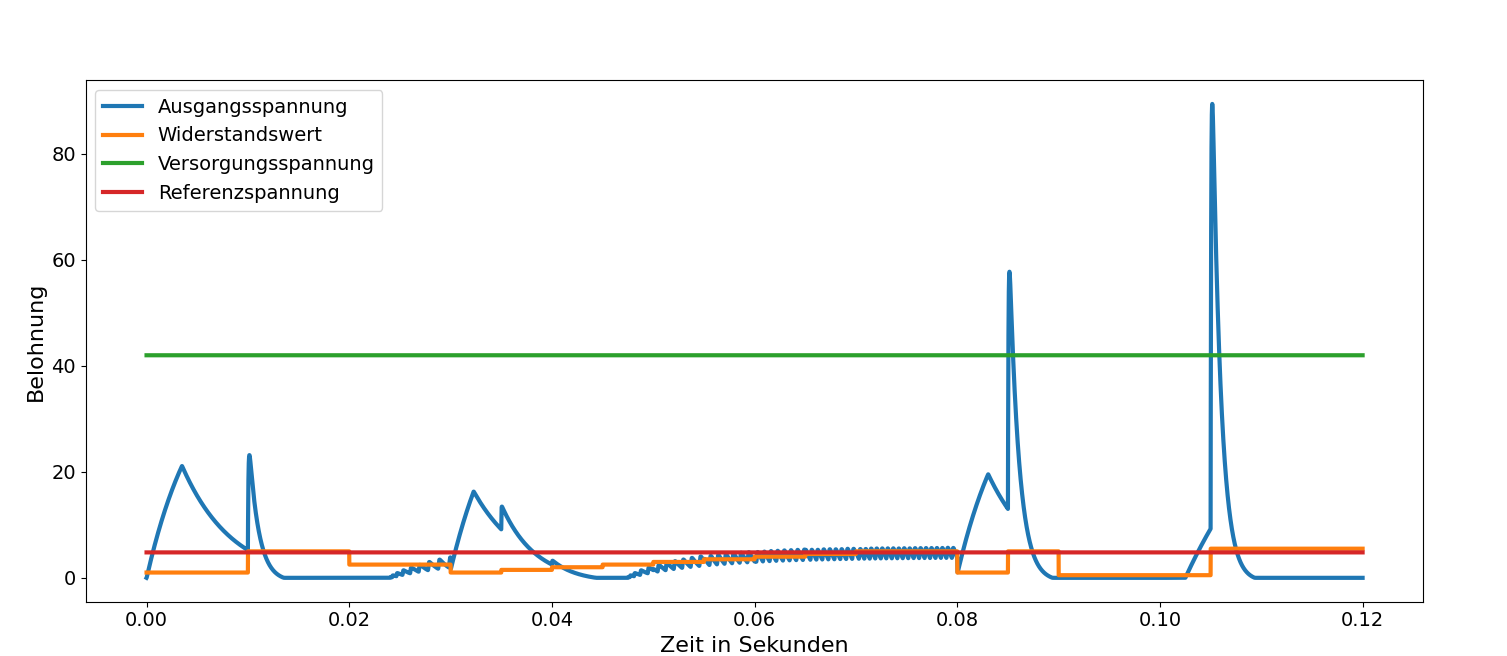
\includegraphics[width=\textwidth]{4Ergebnisse/Phasen/2Phase/5_I.png}
\caption{Stichprobe des Modells Morpheus bei Iteration 0 / Batchfüllung}
\label{fig:untrained}
\end{figure}


Die erste Stichprobe zeigt die Anfangsversuche des PID-Reglers, eine Regelung durchzuführen. Wie in Abbildung \ref{fig:untrained} erkennbar, gelingt es dem Regler noch nicht, die Ausgangsspannung effektiv zu stabilisieren. Die blaue Linie, die die Ausgangsspannung darstellt, haftet nicht an der roten Referenzlinie, was auf eine unzureichende Steuerung hinweist. Insbesondere bei großen Stromspitzen überschreitet die Spannung die Versorgungsspannung und erreicht Werte bis zu 90 Volt, manchmal fällt sie auch auf null ab. Dies würde normalerweise als suboptimales Regelverhalten eingestuft.

Trotzdem, wenn die Störungen nicht zu groß sind und dem System ausreichend Zeit gegeben wird, beginnt es, sich auf den gewünschten Wert einzupendeln, obwohl noch starke Oszillationen sichtbar sind. Dies deutet darauf hin, dass das System das Potenzial hat, sich zu stabilisieren, obwohl der aktuelle Regelungsansatz noch verbesserungsbedürftig ist.
